% ---------------------------------------------------------------------
\chapter{Implementation}
% ---------------------------------------------------------------------
\section{How to Multiple}
Step 0: Environment set up.\\
 Install the Intel RealSense SDK 2.0 (librealsense) for Linux* following the instructions here(https://github.com/IntelRealSense/librealsense/blob/master/doc/installation.md).\\
Install the ROS (not ROS 2) wrapper for librealsense from here(https://github.com/IntelRealSense/realsense-ros/releases).\\
 It is recommended to follow this set of instructions for the installation(https://github.com/IntelRealSense/realsense-ros/blob/development/.travis.yml).\\

Step 1: Obtaining the camera serial numbers.\\
1. Open terminal and change directory to catkin-ws\\
2. Make sure only cam-1 is connected and start the realsense2-camera wrapper:\\
roslaunch realsense2-camera rs-camera.launch\\
Note the serial number it finds in the following log line:\\
$[INFO]$ [1538983051.813336379]: setupDevice...\\
$[INFO]$ [1538983051.813399792]: JSON file is not provided\\
$[INFO]$ [1538983051.813427820]: ROS Node Namespace: camera\\
$[INFO]$ [1538983051.813442869]: Device Name: Intel RealSense D435\\
$[INFO]$ [1538983051.813605893]: Device Serial No: 618206002406\\
$[INFO]$ [1538983051.813622583]: Device FW version: 05.10.03.00\\
The serial number in this case is 618206002406.\\
Record this somewhere and terminate the node using CTRL+C.\\
Repeat the step with now only cam-2 connected.\\
   camera right : 618206002406\\
   camera left  : 617205002698\\
   
   
Step 2: Start both cameras.\\
Open terminal windows (and change directory to catkin-ws directory)$\colon$\\
roslaunch pcl-filter set-transform.launch\\


\begin{figure}[htp]
	\centering % 图片居中
	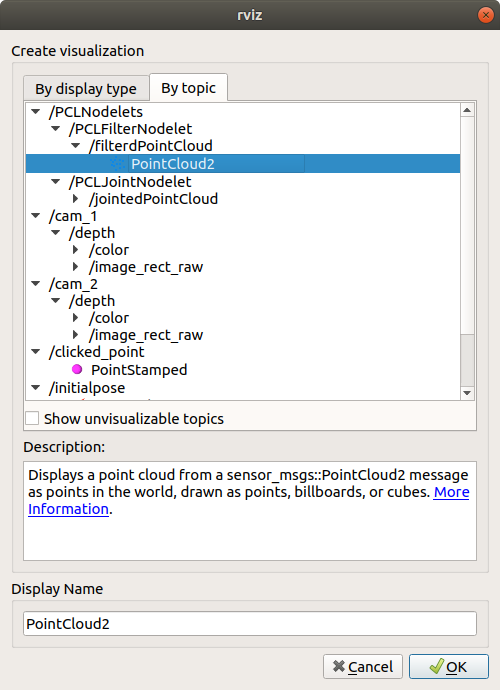
\includegraphics[width = 5.3cm]{figures/topic}
	\caption{Add PointCloud2}
	\label{fig:figure1label}
\end{figure}

Step 3: Publish spatial connection between cameras.\\
The following script calculates the transformation between the 2 cameras from the given parameters and publish the frame transformation.\\
Open a d terminal window – terminal 2 – and enter the following: sh ~/catkin-ws/src/pcl-filter/script/get-transform-info.sh\\


Step 4: Visualizing the point clouds and fine-tune the camera calibration.\\


In the RViz window, do the following:\\
1. Set “Fixed Frame” to “cam-1-link”\\
2. Add -> By topic -> /cam-1/depth/color/points/PointCloud2\\
3. Add -> By topic -> /cam-2/depth/color/points/PointCloud2\\
Now both point clouds are shown together. If you looked closely it’s easy to see that the clouds are not exactly in position. Some features are duplicated. Now it’s time for fine calibration.\\

Switch to terminal 2, where set-cams-transforms.py is still running. Use it to fine-calibrate cam-2 relative to cam-1. The instructions are printed by the program:\\

Use given initial values.\\
Press the following keys to change mode: x, y, z, (a)zimuth, (p)itch, (r)oll\\
For each mode, press 6 to increase by step and 4 to decrease\\
Press + to multiply step by 2 or - to divide\\
Press Q to quit\\



In the meanwhile, after a lot of fiddling around, I was relatively satisfied with the following numbers:\\
x:0.71875 + 0.50625\\
y:-0.1375 + 0.60625\\
z:0.5406250\\
a:-20.625 - 84.0\\
p:108.18750\\
r:-209.5\\
Output:\\

\begin{figure}[htp]
	\centering % 图片居中
	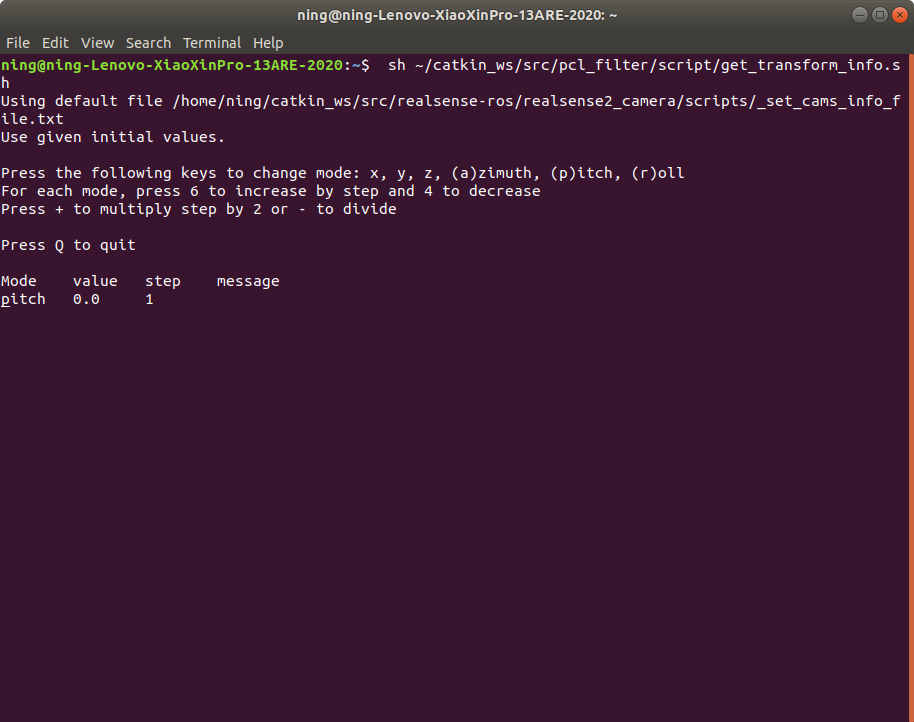
\includegraphics[width = 10.3cm]{figures/set}
	\caption{Set transform}
	\label{fig:figure1label}
\end{figure}
   ~/catkin-ws/src/realsense-ros/realsense2-camera/scripts/-set-cams-info-file.txt\\
\begin{figure}[htp]
	\centering % 图片居中
	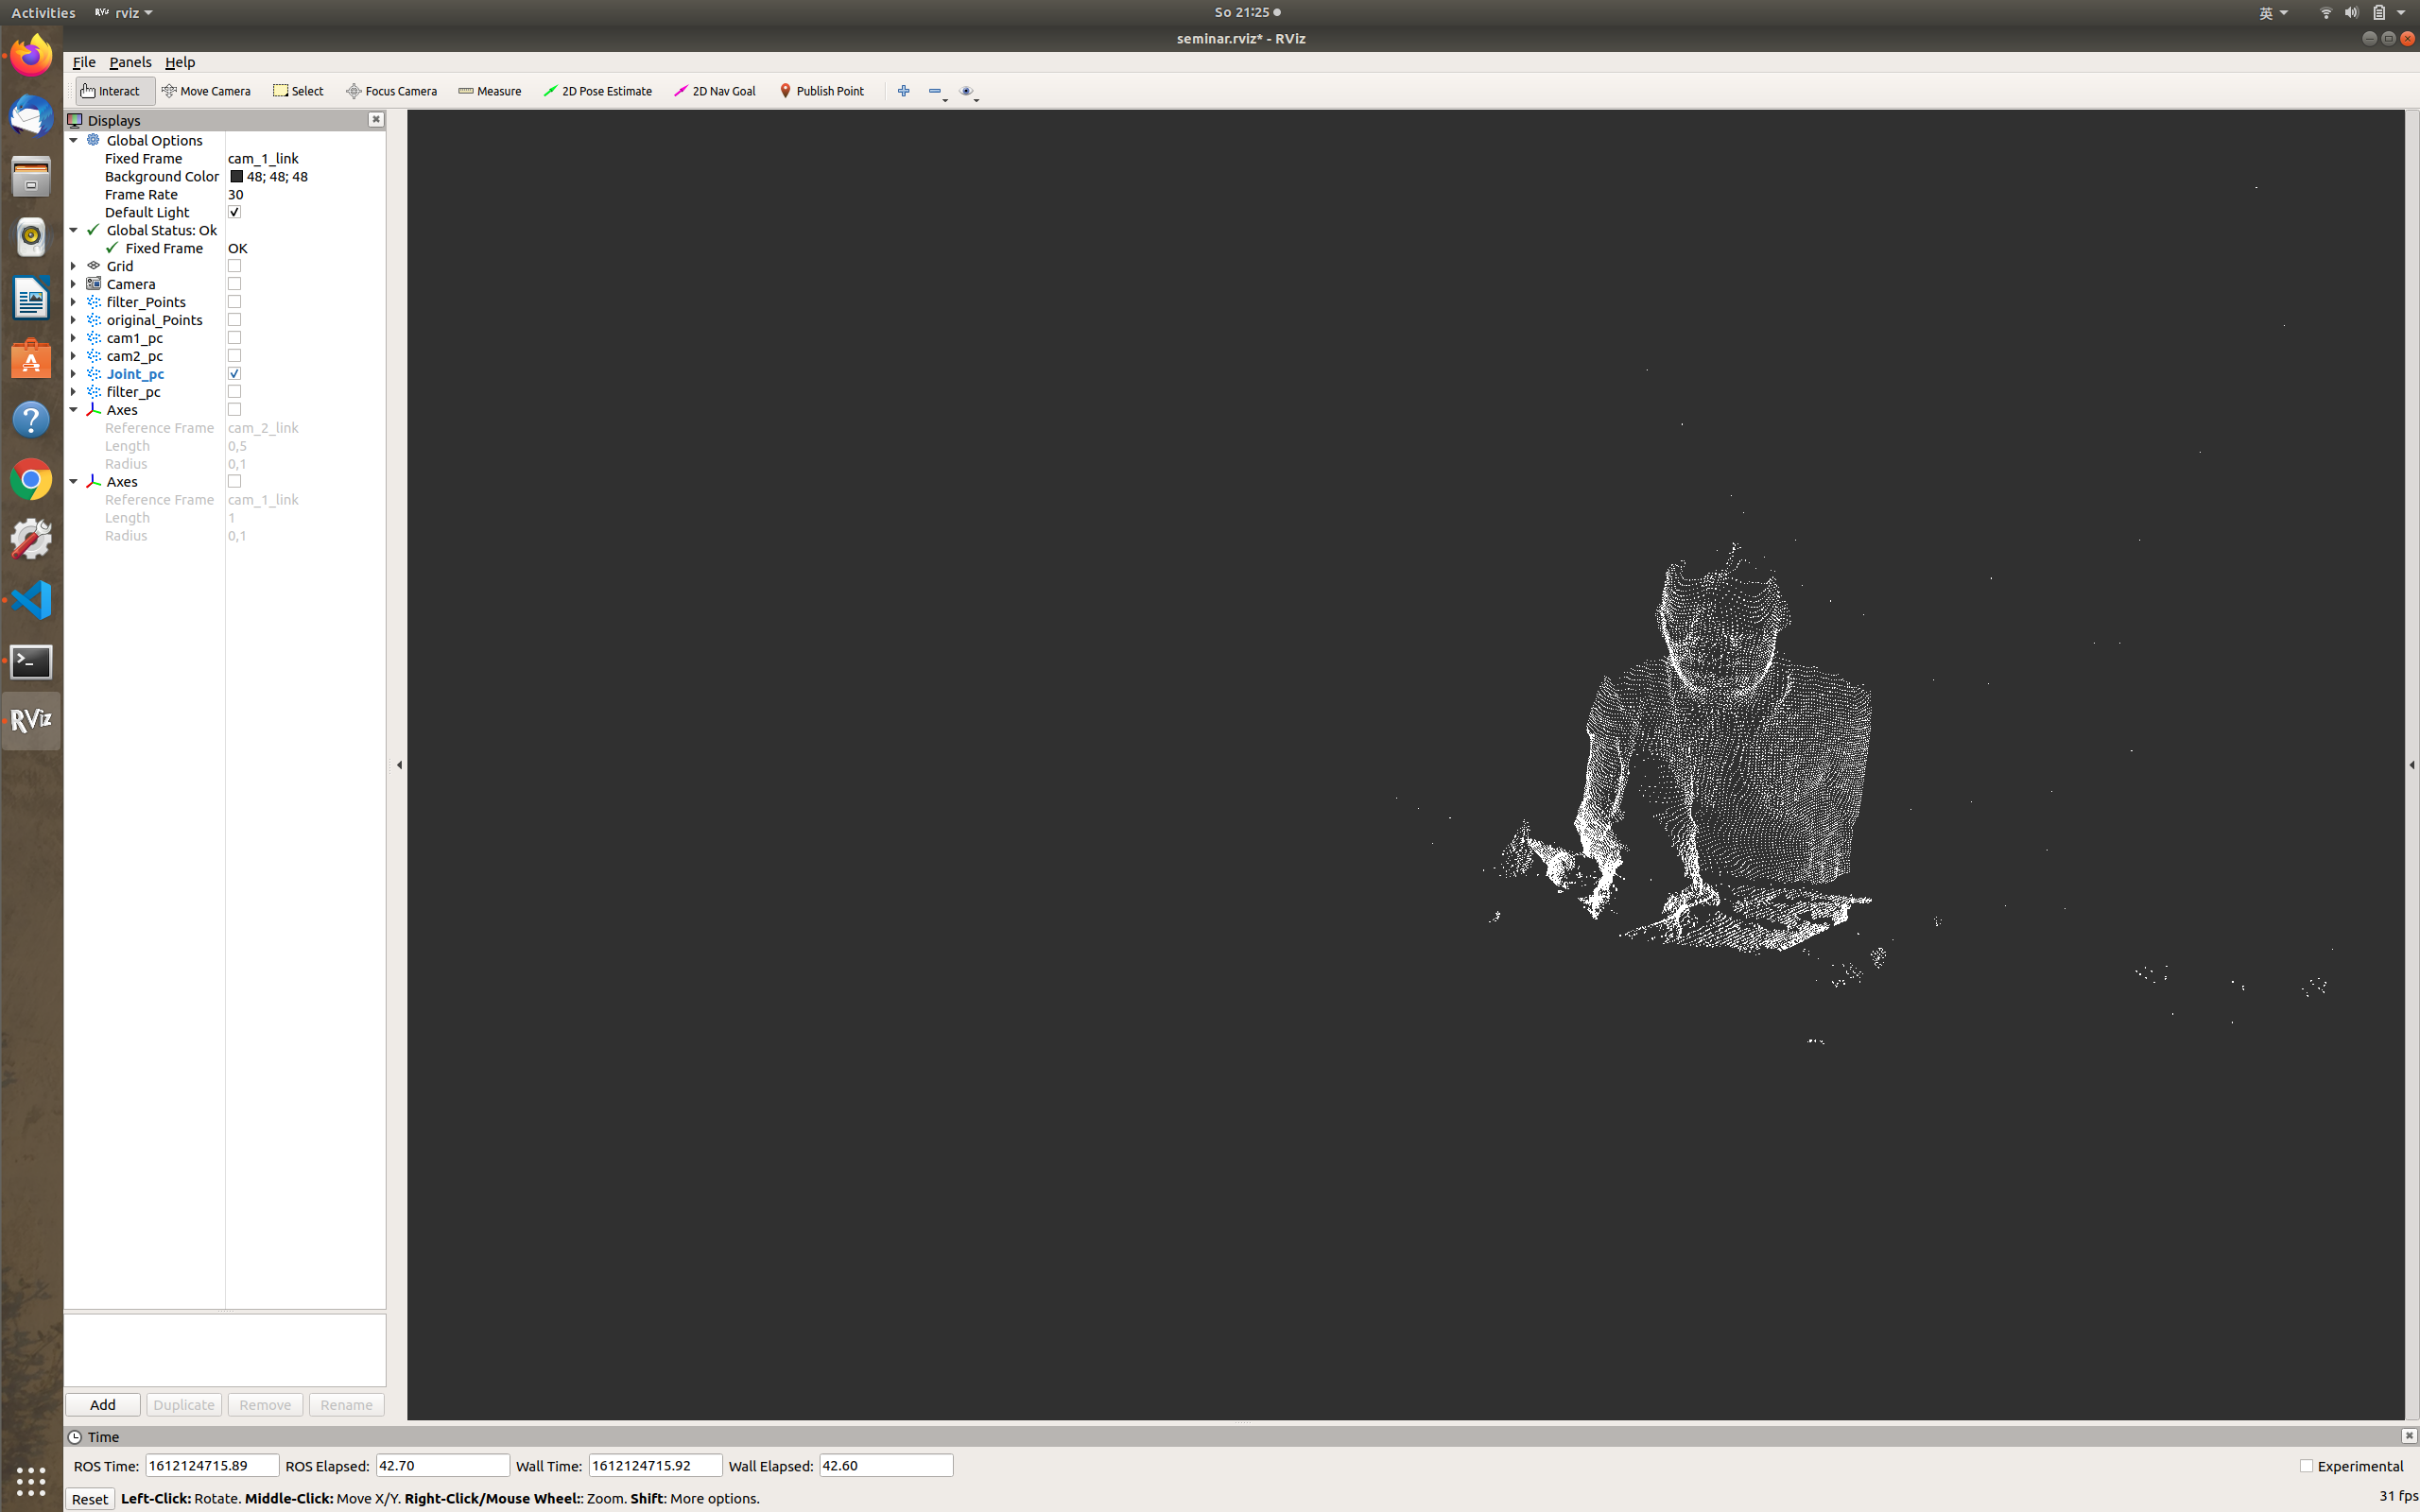
\includegraphics[width = 10.3cm]{figures/final}
	\caption{ the final figure}
	\label{fig:figure1label}
\end{figure}
step 5:
Finally, we will write the obtained coordinate numbers into our code, so that we can complete the point cloud synthesis:\\
roslaunch pcl-filter two-cameras-filter.launch\\




\section{ICP(Iterative Closest Point)}
In this experiment, it is necessary to unify the alternative or multiple sets of point clouds at different angles (ie different reference coordinates) into a unified coordinate system for point cloud registration. In the registration algorithm, we use the ICP algorithm.\\
\begin{figure}[htp]
	\centering % 图片居中
	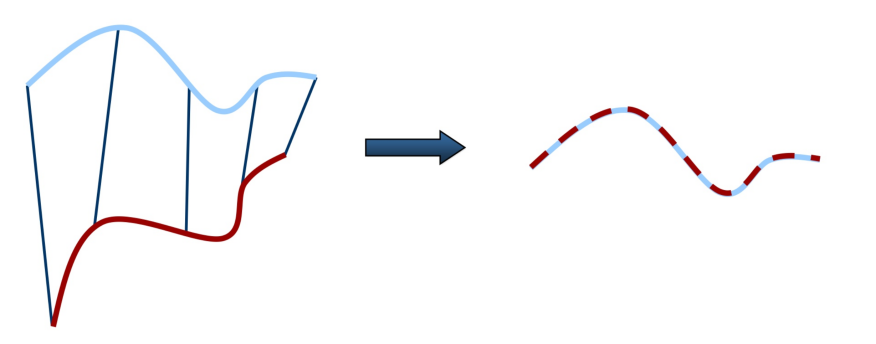
\includegraphics[width = 5.3cm]{figures/icp}
	\caption{ Effektbild of ICP}
	\label{fig:figure1label}
\end{figure}
The basic principle of the ICP algorithm is: in the target point cloud P and source point cloud Q with matching, find the nearest neighbor points (pi, qi) according to certain constraints, and then calculate the optimal matching parameters R and t, The error function is E$\left(R,t\right)$:
$$E\left(R,t\right)=\frac 1n\sum_{i=1}^n \Vert q_i-(Rq_i+t)\Vert^2$$
Where n is the number of nearest neighbor point pairs, $p_i$ is a point in the target point cloud P, $q_i$ is the nearest point corresponding to $p_i$ in the source point cloud Q, R is the rotation matrix, and t is the translation vector.\\

Where n is the number of nearest point pairs, $p_i$ is a point in the target point cloud P, $q_i$ is the closest point corresponding to $p_i$ in the source point cloud Q, R is the rotation matrix, and t is the translation vector.\\

ICP algorithm steps:\\
(1) Take the point set $p_i$ $\in$P in the target point cloud P;\\
(2) Find the corresponding point set $q_i$ $\in$Q in the source point cloud Q, such that $\Vert q_i-p_i\Vert$=min;\\
(3) Calculate the rotation matrix R and the translation matrix t to minimize the error function;\\
(4) Use the rotation matrix R and the translation matrix t obtained in the previous step to rotate and translate $p_i$ to the new one Corresponding point set $p_{i}^{’}=(p_{i}^{’}=Rp_{i}+t,p_{i} \in P)$;\\$$d=\frac 1n\sum_{i=1}^n \Vert p_{i}^{'}-q_i)\Vert^2$$
(5) Calculate the average distance between $p_{i}^{'}$ and the corresponding point set $q_{i}$;\\
(6) If d is less than a given threshold or greater than the preset maximum number of iterations, stop the iterative calculation.Otherwise, return to step 2 until the convergence condition is met.\\

Key points of ICP algorithm:\\
(1) Collection of original point set Uniform sampling, random sampling and normal sampling\\
(2) Determine the corresponding point set Point to point, point to projection, point to surface\\
(3) Calculate the change matrix Quaternion method, SVD singular value decomposition method\\

\section{Rotation matrix}
In this experiment, two or more sets of point clouds under different viewing angles, that is, different reference coordinates, should be unified into a unified coordinate system to perform point cloud registration. First, a rotation matrix is needed to convert one group of point clouds to the coordinate system of another group of point clouds. The rotation matrix is a matrix that has the effect of changing the direction of the vector but not the size when multiplied by a vector and maintaining the chirality.\\
I have already written the rotation matrix in the code, so I don’t need to rotate again, I just need to substitute the data.\\

\section{pcl::SACSegmentation< PointT >}
The class SACSegmentation<PointT> uses the incoming sample consistency algorithm to realize the segmentation class and defines all related function interfaces. The input of this class is to set the model type and related parameters to be segmented, and the output is the final estimated model parameters and segmentation. The obtained interior point set can be divided into different types of objects contained in the point cloud by using different models, such as the segmentation and extraction of straight lines, planes, cylinders, spheres, etc. It is very convenient and robust in the field of automatic recognition and extraction of robots. Sex is also very good.
\section{Transform}
The ‘tf‘ package [Ros] is used to maintain a transformation tree. This transformation
tree contains different frames which corresponds to different coordinate systems. The
’tf’ package allows to get transformation matrices between different frames in the
tree and transform for example vectors from on frame into another. The ‘tf‘ package
is used to keep track about the position of the robot and therefore of the camera
mounted to it.
